%=====================================================================
%  Advanced Optimization  --  Chapter 7  (12pt edition, v3)
%  Nocedal & Wright, Chapter 7: Large-Scale Unconstrained Optimization
%  7.1 inexact Newton (forcing sequence, Newton-CG, CG-Steihaug, Lanczos)
%  7.2 limited-memory quasi-Newton (L-BFGS, memoryless BFGS, compact form)
%  7.3 sparse quasi-Newton updates
%  7.4 partially separable functions
%  7.5 perspectives and software (in the summary table)
%
%  Layout rules for this deck (30 slides)
%   - body 12pt; nothing in the body below 10pt; footline 8pt
%   - one theorem per slide, or at most three displayed equations
%   - proofs are omitted; a red "Read:" pointer gives the pages in the book
%   - equation numbers and theorem statements follow the book
%   - material that is not in the book is marked "(Not in the book.)"
%   - no [shrink] option anywhere
%=====================================================================
\documentclass[aspectratio=169,12pt]{beamer}

\usetheme{default}
\usecolortheme{seahorse}
\useinnertheme{rectangles}
\setbeamersize{text margin left=7mm,text margin right=7mm}
\setbeamertemplate{navigation symbols}{}
\setbeamerfont{title}{series=\bfseries,size=\LARGE}
\setbeamerfont{subtitle}{size=\large}
\setbeamerfont{institute}{size=\small}
\setbeamerfont{frametitle}{series=\bfseries,size=\large}
\setbeamerfont{block title}{series=\bfseries,size=\normalsize}
\setbeamerfont{footline}{size=\scriptsize}   % 8pt at 12pt base
\setbeamercolor{frametitle}{fg=black!85,bg=black!5}
\setbeamercolor{block title}{bg=structure!25,fg=black!85}
\setbeamercolor{block body}{bg=structure!8}
\setbeamercolor{alerted text}{fg=red!65!black}
\setbeamercolor{footline}{fg=black!60}
\setbeamertemplate{itemize item}{\small$\blacktriangleright$}
\setbeamertemplate{itemize subitem}{\footnotesize$-$}
\setbeamertemplate{enumerate items}[default]
\setbeamerfont{enumerate item}{size=\normalsize,series=\bfseries}
\setbeamertemplate{footline}{%
  \leavevmode\hbox to\paperwidth{\hskip7mm\usebeamerfont{footline}\usebeamercolor[fg]{footline}%
  \insertsection\hfill\insertframenumber\,/\,\inserttotalframenumber\hskip7mm}\vskip2.2mm}

\usepackage{amsmath,amssymb}
\usepackage{booktabs}
\usepackage{tikz}
% no math subscript below 8pt, also inside \small and \footnotesize text
\DeclareMathSizes{12}{12}{8}{8}
\DeclareMathSizes{10.95}{10.95}{8}{8}
\DeclareMathSizes{10}{10}{8}{8}

\newcommand{\R}{\mathbb{R}}
\newcommand{\xs}{x^{*}}
\newcommand{\gradf}{\nabla f}
\newcommand{\hessf}{\nabla^{2} f}
\newcommand{\la}{\leftarrow}
\newcommand{\eqn}[1]{\text{\small(#1)}}
% reading pointer to the book (page numbers: Nocedal & Wright, 2nd ed.)
\newcommand{\readbook}[1]{{\color{red}\textbf{Read:} #1}}
% marker for material that is not in the book
\newcommand{\notinbook}{{\small(Not in the book.)}}
% algorithm listing: statement | equation number
\newcommand{\algostretch}{1.12}
\newenvironment{algo}{\par\renewcommand{\arraystretch}{\algostretch}%
  \begin{tabular}{@{}l@{\hspace{2.2em}}l@{}}}{\end{tabular}\par}

\title{Advanced Optimization}
\subtitle{Chapter 7 --- Large-Scale Unconstrained Optimization}
\author{Hongseok Kim}
\institute{Department of Electronic Engineering, Sogang University}
\date{Fall 2026}


\begin{document}

\section{Chapter 7: introduction}

\begin{frame}
  \titlepage
  \begin{center}\small
    Reading: Nocedal \& Wright, \emph{Numerical Optimization}, 2nd ed., Chapter 7
  \end{center}
\end{frame}

\begin{frame}{Large-scale unconstrained optimization}
  Thousands or millions of variables: the \alert{storage} and \alert{computational cost} of the
  algorithm must be kept at a tolerable level.

  \vspace{0.3em}
  \begin{center}
  \small\setlength\tabcolsep{5pt}
  \begin{tabular}{lll}
    \toprule
    Section & Approach & Idea \\
    \midrule
    \S7.1 & Inexact Newton & approximate Newton step by CG or Lanczos \\
    \S7.2 & Limited-memory quasi-Newton & a few vectors of length $n$ instead of a matrix \\
    \S7.3 & Sparse quasi-Newton & $B_{k}$ with the sparsity pattern of the Hessian \\
    \S7.4 & Partial separability & $f$ is a sum of element functions \\
    \bottomrule
  \end{tabular}
  \end{center}

  \begin{itemize}\setlength\itemsep{0.3em}
    \item If a sparse factorization of the Hessian is affordable, Newton methods based on
      sparse factorizations are effective.
    \item Nonlinear CG (\S5.2) applies to large problems without modification.
  \end{itemize}
\end{frame}

%=====================================================================
\section{\S7.1 Inexact Newton: local convergence}

\begin{frame}{Inexact Newton methods}
  The Newton step $p_{k}^{N}$ solves the symmetric $n\times n$ linear system
  \[ \hessf_{k}\,p_{k}^{N}=-\gradf_{k} . \tag{7.1} \]
  Solve (7.1) approximately by CG or Lanczos. Residual of the inexact Newton step $p_{k}$:
  \[ r_{k}=\hessf_{k}\,p_{k}+\gradf_{k} . \tag{7.2} \]
  Terminate the iterative solver when
  \[ \|r_{k}\|\le\eta_{k}\|\gradf_{k}\| , \tag{7.3} \]
  where $\{\eta_{k}\}$, with $0<\eta_{k}<1$ for all $k$, is the \textbf{forcing sequence}.
  No factorization of $\hessf_{k}$ is needed.
\end{frame}

\begin{frame}{Theorem 7.1: local convergence}
  \begin{block}{Theorem 7.1}
    Suppose that $\hessf(x)$ exists and is continuous in a neighborhood of a minimizer $\xs$,
    with $\hessf(\xs)$ positive definite. Consider the iteration $x_{k+1}=x_{k}+p_{k}$ where
    $p_{k}$ satisfies (7.3), and assume that $\eta_{k}\le\eta$ for some constant $\eta\in[0,1)$.
    Then, if the starting point $x_{0}$ is sufficiently near $\xs$, the sequence $\{x_{k}\}$
    converges to $\xs$ and satisfies
    \[ \|\hessf(\xs)(x_{k+1}-\xs)\|\le\hat\eta\,\|\hessf(\xs)(x_{k}-\xs)\| , \tag{7.4} \]
    for some constant $\hat\eta$ with $\eta<\hat\eta<1$.
  \end{block}

  Local convergence only requires that $\eta_{k}$ is bounded away from $1$.\\
  The book gives an informal derivation, not a rigorous proof. \readbook{pp.~166--167.}
\end{frame}

\begin{frame}{Theorem 7.2: the forcing sequence determines the rate}
  \[
    \text{From the derivation of Theorem 7.1:}\qquad
    \frac{\|\gradf_{k+1}\|}{\|\gradf_{k}\|}\le\eta_{k}+o(1) .
    \tag{7.8}
  \]

  \begin{block}{Theorem 7.2}
    Suppose that the conditions of Theorem 7.1 hold, and assume that the iterates $\{x_{k}\}$
    generated by the inexact Newton method converge to $\xs$. Then the rate of convergence
    is superlinear if $\eta_{k}\to 0$. If in addition, $\hessf(x)$ is Lipschitz continuous for $x$
    near $\xs$ and if $\eta_{k}=O(\|\gradf_{k}\|)$, then the convergence is quadratic.
  \end{block}

  \begin{itemize}\setlength\itemsep{0.25em}
    \item $\eta_{k}=\min\big(0.5,\sqrt{\|\gradf_{k}\|}\big)$: superlinear.\quad
      $\eta_{k}=\min(0.5,\|\gradf_{k}\|)$: quadratic.
    \item The results are local and assume the unit step $\alpha_{k}=1$.
      \readbook{pp.~167--168.}
  \end{itemize}
\end{frame}

%=====================================================================
\section{\S7.1 Inexact Newton: Newton--CG}

\begin{frame}{Line search Newton--CG (truncated Newton)}
  Apply the CG method to the Newton equations, written as
  \[ B_{k}p=-\gradf_{k},\qquad B_{k}=\hessf_{k}, \tag{7.9} \]
  and stop by a test of the form (7.3). Inner CG iteration: directions $d_{j}$, iterates $z_{j}$.

  \vspace{0.3em}
  CG requires a positive definite matrix, and $\hessf_{k}$ may have negative eigenvalues.
  Differences from Algorithm 5.2:
  \begin{itemize}\setlength\itemsep{0.3em}
    \item the starting point is $z_{0}=0$;
    \item a positive tolerance $\epsilon_{k}$ lets CG terminate at an inexact solution;
    \item the \alert{negative curvature test} $d_{j}^{T}B_{k}d_{j}\le 0$ ensures that $p_{k}$ is a descent
      direction. If it holds at $j=0$, the method returns $p_{k}=-\gradf_{k}$.
  \end{itemize}
\end{frame}

\begin{frame}{Algorithm 7.1 (line search Newton--CG)}
  \begin{block}{}\small
    \begin{algo}
      Given initial point $x_{0}$ & \\
      \textbf{for} $k=0,1,2,\dots$ & \\
      \quad define tolerance $\epsilon_{k}=\min\big(0.5,\sqrt{\|\gradf_{k}\|}\big)\,\|\gradf_{k}\|$ & \\
      \quad set $z_{0}=0$,\ \ $r_{0}=\gradf_{k}$,\ \ $d_{0}=-r_{0}=-\gradf_{k}$ & \\
      \quad \textbf{for} $j=0,1,2,\dots$ & \\
      \qquad \textbf{if} $d_{j}^{T}B_{k}d_{j}\le 0$:\ \ \textbf{if} $j=0$ \textbf{return} $p_{k}=-\gradf_{k}$;\ \
             \textbf{else return} $p_{k}=z_{j}$ & \\
      \qquad set $\alpha_{j}=r_{j}^{T}r_{j}/d_{j}^{T}B_{k}d_{j}$;\ \ $z_{j+1}=z_{j}+\alpha_{j}d_{j}$;\ \
             $r_{j+1}=r_{j}+\alpha_{j}B_{k}d_{j}$ & \\
      \qquad \textbf{if} $\|r_{j+1}\|<\epsilon_{k}$ \textbf{return} $p_{k}=z_{j+1}$ & \\
      \qquad set $\beta_{j+1}=r_{j+1}^{T}r_{j+1}/r_{j}^{T}r_{j}$;\ \ $d_{j+1}=-r_{j+1}+\beta_{j+1}d_{j}$ & \\
      \quad set $x_{k+1}=x_{k}+\alpha_{k}p_{k}$, where $\alpha_{k}$ satisfies the Wolfe, Goldstein, or
            Armijo & \\
      \qquad backtracking conditions (using $\alpha_{k}=1$ if possible) & \\
    \end{algo}
  \end{block}
\end{frame}

\begin{frame}{Algorithm 7.1: weakness, and Hessian-free implementation}
  \begin{itemize}\setlength\itemsep{0.5em}
    \item \textbf{Weakness.} When $\hessf_{k}$ is nearly singular, the direction can be long and
      of poor quality: many function evaluations in the line search, small reduction in $f$.
      The trust-region Newton--CG method handles this more effectively.
    \item \textbf{Hessian-free.} The algorithm needs only products $\hessf_{k}d$, not the matrix.
      With a small differencing interval $h$:
  \end{itemize}
  \[ \hessf_{k}d\approx\frac{\gradf(x_{k}+hd)-\gradf(x_{k})}{h} . \tag{7.10} \]
  The accuracy is $O(h)$. Price: \alert{one new gradient evaluation per CG iteration}.\\
  Automatic differentiation (Chapter 8) gives $\hessf_{k}d$ exactly, at about 12 times the cost
  of $f$, independent of $n$. \readbook{\S8.2, pp.~215--216.}\
  \notinbook\ \texttt{jvp(grad f)} in JAX, \texttt{torch.func} in PyTorch:
  Newton--CG without ever forming the Hessian.

  \vspace{0.2em}
  The CG iteration can be preconditioned as in Chapter 5.
\end{frame}

\begin{frame}{Trust-region Newton--CG}
  Trust-region subproblem, with $B_{k}=\hessf_{k}$:
  \[
    \min_{p\in\R^{n}}\ m_{k}(p)\overset{\text{def}}{=}f_{k}+(\gradf_{k})^{T}p+\tfrac12p^{T}B_{k}p
    \qquad\text{subject to }\|p\|\le\Delta_{k} .
    \tag{7.11}
  \]
  Algorithm 7.2 (Steihaug) is CG started from $z_{0}=0$, with three ways to stop:
  \begin{enumerate}\setlength\itemsep{0.3em}
    \item $d_{j}^{T}B_{k}d_{j}\le 0$ (nonpositive curvature): move along $d_{j}$ to the boundary;
    \item $\|z_{j+1}\|\ge\Delta_{k}$: stop at the intersection with the boundary;
    \item $\|r_{j+1}\|<\epsilon_{k}$: return $z_{j+1}$.
  \end{enumerate}

  \vspace{0.3em}
  The step $p_{k}$ is used in Algorithm 4.1. Near a well-behaved solution the bound is
  inactive, and the method reduces to the inexact Newton method of Theorems 7.1, 7.2.
\end{frame}

\begin{frame}{Algorithm 7.2 (CG--Steihaug)}
  \renewcommand{\algostretch}{1.0}%
  \begin{block}{}\small
    \begin{algo}
      Given tolerance $\epsilon_{k}>0$;\ \ set $z_{0}=0$,\ \ $r_{0}=\gradf_{k}$,\ \ $d_{0}=-r_{0}=-\gradf_{k}$ & \\
      \textbf{if} $\|r_{0}\|<\epsilon_{k}$ \textbf{return} $p_{k}=z_{0}=0$ & \\
      \textbf{for} $j=0,1,2,\dots$ & \\
      \quad \textbf{if} $d_{j}^{T}B_{k}d_{j}\le 0$ & \\
      \qquad find $\tau$ such that $p_{k}=z_{j}+\tau d_{j}$ minimizes $m_{k}(p_{k})$ in (4.5) & \\
      \qquad and satisfies $\|p_{k}\|=\Delta_{k}$;\ \ \textbf{return} $p_{k}$ & \\
      \quad set $\alpha_{j}=r_{j}^{T}r_{j}/d_{j}^{T}B_{k}d_{j}$;\ \ $z_{j+1}=z_{j}+\alpha_{j}d_{j}$ & \\
      \quad \textbf{if} $\|z_{j+1}\|\ge\Delta_{k}$ & \\
      \qquad find $\tau\ge 0$ such that $p_{k}=z_{j}+\tau d_{j}$ satisfies $\|p_{k}\|=\Delta_{k}$;\ \
             \textbf{return} $p_{k}$ & \\
      \quad set $r_{j+1}=r_{j}+\alpha_{j}B_{k}d_{j}$ & \\
      \quad \textbf{if} $\|r_{j+1}\|<\epsilon_{k}$ & \\
      \qquad \textbf{return} $p_{k}=z_{j+1}$ & \\
      \quad set $\beta_{j+1}=r_{j+1}^{T}r_{j+1}/r_{j}^{T}r_{j}$;\ \ $d_{j+1}=-r_{j+1}+\beta_{j+1}d_{j}$ & \\
    \end{algo}
  \end{block}
\end{frame}

\begin{frame}{Theorem 7.3: two properties of Algorithm 7.2}
  \begin{itemize}\setlength\itemsep{0.3em}
    \item The initialization $z_{0}=0$ is crucial. If $\|\gradf_{k}\|_{2}\ge\epsilon_{k}$, then
      $m_{k}(p_{k})\le m_{k}(p_{k}^{C})$: the step is at least as good as the Cauchy point, so the
      method is globally convergent.
  \end{itemize}

  \begin{block}{Theorem 7.3}
    The sequence of vectors $\{z_{j}\}$ generated by Algorithm 7.2 satisfies
    \[ 0=\|z_{0}\|_{2}<\cdots<\|z_{j}\|_{2}<\|z_{j+1}\|_{2}<\cdots<\|p_{k}\|_{2}\le\Delta_{k} . \]
  \end{block}

  \begin{itemize}\setlength\itemsep{0.3em}
    \item It is therefore acceptable to stop as soon as the boundary is reached: no later
      iterate with a lower value of $m_{k}$ lies inside the trust region.
    \item \readbook{proof of Theorem 7.3 (uses Theorem 5.2), pp.~172--173.}
  \end{itemize}
\end{frame}

\begin{frame}{Preconditioning the trust-region Newton--CG method}
  \setlength{\abovedisplayskip}{5pt}\setlength{\belowdisplayskip}{5pt}%
  Nonsingular $D$; the trust region is defined in the scaled norm:
  \[
    \min_{p\in\R^{n}}\ m_{k}(p)\overset{\text{def}}{=}f_{k}+\gradf_{k}^{T}p+\tfrac12p^{T}B_{k}p
    \qquad\text{subject to }\|Dp\|\le\Delta_{k} .
    \tag{7.13}
  \]
  Change of variables $\hat p=Dp$, as in (5.37)--(5.38) with $D$ in the role of $C$:
  \[
    \gradf_{k}^{T}p=(D^{-T}\gradf_{k})^{T}\hat p,\qquad
    p^{T}B_{k}p=\hat p^{T}(D^{-T}B_{k}D^{-1})\hat p,\qquad
    \|Dp\|=\|\hat p\| .
  \]
  The preconditioned subproblem, with $\hat g_{k}=D^{-T}\gradf_{k}$ and $\hat B_{k}=D^{-T}B_{k}D^{-1}$:
  \[
    \min_{\hat p\in\R^{n}}\ \hat m_{k}(\hat p)=f_{k}+\hat g_{k}^{T}\hat p+\tfrac12\hat p^{T}\hat B_{k}\hat p
    \qquad\text{subject to }\|\hat p\|\le\Delta_{k} .
  \]
  This has exactly the form (7.11): Algorithm 7.2 applies with $(\hat g_{k},\hat B_{k})$; $p_{k}=D^{-1}\hat p_{k}$.
  CG speed is now set by the eigenvalues of $\hat B_{k}$. $D=L^{T}$ from incomplete Cholesky,
  shifted by Algorithm 7.3 ($LL^{T}=\bar B+\alpha_{k}I$) if $\hessf_{k}$ is indefinite. \readbook{pp.~174--175.}
\end{frame}

\begin{frame}{Trust-region Newton--Lanczos}
  Algorithm 7.2 accepts \emph{any} direction of negative curvature, even when it gives an
  insignificant reduction in the model. Example:
  \[ \min_{p}\ m(p)=10^{-3}p_{1}-10^{-4}p_{1}^{2}-p_{2}^{2}\qquad\text{subject to }\|p\|\le 1 . \]
  Steepest descent at $p=0$ is $(-10^{-3},0)^{T}$: reduction about $10^{-3}$. Along $e_{2}$: about $1$.

  \vspace{0.3em}
  \textbf{Lanczos} instead of CG: after $j$ steps, $Q_{j}$ ($n\times j$, orthogonal columns spanning
  the Krylov subspace) with $Q_{j}^{T}BQ_{j}=T_{j}$ tridiagonal. Solve
  \[
    \min_{w\in\R^{j}}\ f_{k}+e_{1}^{T}Q_{j}(\gradf_{k})\,e_{1}^{T}w+\tfrac12w^{T}T_{j}w
    \qquad\text{subject to }\|w\|\le\Delta_{k} ,
    \tag{7.14}
  \]
  and set $p_{k}=Q_{j}w$. More robust; the subproblem is more expensive.

  \vspace{0.2em}
  {\small(Lanczos is not covered in this course; the example above is the point.)}
\end{frame}

%=====================================================================
\section{\S7.2 Limited-memory quasi-Newton: L-BFGS}

\begin{frame}{Limited-memory quasi-Newton methods}
  For large problems whose Hessian cannot be computed at a reasonable cost or is not
  sparse. Recall the BFGS method (Algorithm 6.1):
  \[ x_{k+1}=x_{k}-\alpha_{k}H_{k}\gradf_{k}, \tag{7.15} \]
  \[ H_{k+1}=V_{k}^{T}H_{k}V_{k}+\rho_{k}s_{k}s_{k}^{T}, \tag{7.16} \]
  \[ \rho_{k}=\frac{1}{y_{k}^{T}s_{k}},\qquad V_{k}=I-\rho_{k}y_{k}s_{k}^{T} . \tag{7.17} \]
  $H_{k}$ is generally dense: storing it is prohibitive when $n$ is large.

  \begin{block}{Idea of L-BFGS}
    Store only the \alert{$m$ most recent pairs} $\{s_{i},y_{i}\}$, and discard the oldest pair at each
    iteration. Modest values of $m$ (between 3 and 20, say) often work well.
  \end{block}
\end{frame}

\begin{frame}{The L-BFGS approximation}
  At iteration $k$ the stored pairs are $\{s_{i},y_{i}\}$, $i=k-m,\dots,k-1$. Choose an initial
  approximation $H_{k}^{0}$ (it may vary from iteration to iteration) and apply (7.16)
  $m$ times:
  \begin{align}
    H_{k}={}&\big(V_{k-1}^{T}\cdots V_{k-m}^{T}\big)\,H_{k}^{0}\,\big(V_{k-m}\cdots V_{k-1}\big) \notag\\
    &+\rho_{k-m}\big(V_{k-1}^{T}\cdots V_{k-m+1}^{T}\big)\,s_{k-m}s_{k-m}^{T}\,\big(V_{k-m+1}\cdots V_{k-1}\big) \notag\\
    &+\rho_{k-m+1}\big(V_{k-1}^{T}\cdots V_{k-m+2}^{T}\big)\,s_{k-m+1}s_{k-m+1}^{T}\,\big(V_{k-m+2}\cdots V_{k-1}\big) \notag\\
    &+\cdots \notag\\
    &+\rho_{k-1}s_{k-1}s_{k-1}^{T} . \tag{7.19}
  \end{align}
  $H_{k}$ is never formed. Only the product $H_{k}\gradf_{k}$ is computed, by a recursion.
\end{frame}

\begin{frame}{Algorithm 7.4 (L-BFGS two-loop recursion)}
  \begin{block}{}
    \begin{algo}
      $q\la\gradf_{k}$ & \\
      \textbf{for} $i=k-1,k-2,\dots,k-m$ & \\
      \qquad $\alpha_{i}\la\rho_{i}s_{i}^{T}q$;\qquad $q\la q-\alpha_{i}y_{i}$ & \\
      $r\la H_{k}^{0}q$ & \\
      \textbf{for} $i=k-m,k-m+1,\dots,k-1$ & \\
      \qquad $\beta\la\rho_{i}y_{i}^{T}r$;\qquad $r\la r+s_{i}(\alpha_{i}-\beta)$ & \\
      \textbf{stop} with result $H_{k}\gradf_{k}=r$ & \\
    \end{algo}
  \end{block}

  Cost: \alert{$4mn$ multiplications}, plus the product $H_{k}^{0}q$ ($n$ multiplications if $H_{k}^{0}$ is
  diagonal). Storage: the $m$ pairs $\{s_{i},y_{i}\}$.
\end{frame}

\begin{frame}{The initial matrix $H_{k}^{0}$ and the line search}
  \begin{itemize}\setlength\itemsep{0.5em}
    \item In Algorithm 7.4 the multiplication by $H_{k}^{0}$ is isolated from the rest of the
      computation. $H_{k}^{0}$ can be chosen freely and can vary between iterations.
    \item A choice that has proved effective in practice: $H_{k}^{0}=\gamma_{k}I$, where
  \end{itemize}
  \[ \gamma_{k}=\frac{s_{k-1}^{T}y_{k-1}}{y_{k-1}^{T}y_{k-1}} . \tag{7.20} \]
  \begin{itemize}\setlength\itemsep{0.5em}
    \item $\gamma_{k}$ is the scaling factor of (6.21): it estimates the size of the true Hessian
      along the most recent search direction. The search direction is then well scaled,
      and $\alpha_{k}=1$ is accepted in most iterations.
    \item The line search should be based on the Wolfe conditions (3.6) or the strong
      Wolfe conditions (3.7), so that BFGS updating is stable.
  \end{itemize}
\end{frame}

\begin{frame}{Algorithm 7.5 (L-BFGS)}
  \begin{block}{}
    \begin{algo}
      Choose starting point $x_{0}$, integer $m>0$;\ \ $k\la 0$ & \\
      \textbf{repeat} & \\
      \qquad choose $H_{k}^{0}$ (for example, by using (7.20)) & \\
      \qquad compute $p_{k}\la-H_{k}\gradf_{k}$ from Algorithm 7.4 & \\
      \qquad compute $x_{k+1}\la x_{k}+\alpha_{k}p_{k}$, where $\alpha_{k}$ satisfies the Wolfe conditions & \\
      \qquad \textbf{if} $k>m$:\ \ discard the vector pair $\{s_{k-m},y_{k-m}\}$ from storage & \\
      \qquad compute and save $s_{k}\la x_{k+1}-x_{k}$,\ \ $y_{k}=\gradf_{k+1}-\gradf_{k}$;\ \ $k\la k+1$ & \\
      \textbf{until} convergence & \\
    \end{algo}
  \end{block}

  During its first $m-1$ iterations, Algorithm 7.5 is equivalent to the BFGS algorithm of
  Chapter 6, if the initial matrix $H_{0}$ is the same and L-BFGS chooses $H_{k}^{0}=H_{0}$.
\end{frame}

\begin{frame}{Performance of L-BFGS (Table 7.1)}
  \begin{center}
  \small\setlength\tabcolsep{5pt}
  \begin{tabular}{lr rr rr rr rr}
    \toprule
    & & \multicolumn{2}{c}{$m=3$} & \multicolumn{2}{c}{$m=5$} & \multicolumn{2}{c}{$m=17$} & \multicolumn{2}{c}{$m=29$} \\
    \cmidrule(lr){3-4}\cmidrule(lr){5-6}\cmidrule(lr){7-8}\cmidrule(lr){9-10}
    Problem & $n$ & nfg & time & nfg & time & nfg & time & nfg & time \\
    \midrule
    DIXMAANL & 1500 & 146 & 16.5 & 134 & 17.4 & 120 & 28.2 & 125 & 44.4 \\
    EIGENALS & 110 & 821 & 21.5 & 569 & 15.7 & 363 & 16.2 & 168 & 12.5 \\
    FREUROTH & 1000 & $>$999 & --- & $>$999 & --- & 69 & 8.1 & 38 & 6.3 \\
    TRIDIA & 1000 & 876 & 46.6 & 611 & 41.4 & 531 & 84.6 & 462 & 127.1 \\
    \bottomrule
  \end{tabular}
  \end{center}

  \begin{itemize}\setlength\itemsep{0.3em}
    \item nfg: function and gradient evaluations. Larger $m$: fewer evaluations, but each
      iteration costs more. The best $m$ is problem dependent.
    \item The rate of convergence is linear. \alert{Main weakness:} slow convergence on
      ill-conditioned problems (Hessian with a wide distribution of eigenvalues).
  \end{itemize}
\end{frame}

\begin{frame}{Relationship with conjugate gradient methods}
  Hestenes--Stiefel direction (5.46), with $s_{k}=\alpha_{k}p_{k}$:
  \[
    p_{k+1}=-\gradf_{k+1}+\frac{\gradf_{k+1}^{T}y_{k}}{y_{k}^{T}p_{k}}\,p_{k}
    =-\Big(I-\frac{s_{k}y_{k}^{T}}{y_{k}^{T}s_{k}}\Big)\gradf_{k+1}\equiv-\hat H_{k+1}\gradf_{k+1} .
    \tag{7.21}
  \]
  $\hat H_{k+1}$ is neither symmetric nor positive definite. Symmetric, positive definite, and
  satisfying the secant equation:
  \[
    H_{k+1}=\Big(I-\frac{s_{k}y_{k}^{T}}{y_{k}^{T}s_{k}}\Big)\Big(I-\frac{y_{k}s_{k}^{T}}{y_{k}^{T}s_{k}}\Big)
    +\frac{s_{k}s_{k}^{T}}{y_{k}^{T}s_{k}} .
    \tag{7.22}
  \]
  \begin{itemize}\setlength\itemsep{0.25em}
    \item (7.22) is one BFGS update of the identity: \alert{memoryless BFGS} ($m=1$, $H_{k}^{0}=I$).
    \item Exact line search: $p_{k+1}=-H_{k+1}\gradf_{k+1}$ is the Hestenes--Stiefel direction \eqn{7.23}.
  \end{itemize}
\end{frame}

%=====================================================================
\section{\S7.2 Limited-memory quasi-Newton: compact representation}

\begin{frame}{Theorem 7.4: compact representation of BFGS updating}
  \begin{block}{Theorem 7.4}\small
    Let $B_{0}$ be symmetric and positive definite, and assume that the $k$ vector pairs
    $\{s_{i},y_{i}\}_{i=0}^{k-1}$ satisfy $s_{i}^{T}y_{i}>0$. Let $B_{k}$ be obtained by applying $k$ BFGS updates
    with these vector pairs to $B_{0}$, using the formula (6.19). We then have that
    \[
      B_{k}=B_{0}-\begin{bmatrix}B_{0}S_{k}&Y_{k}\end{bmatrix}
      \begin{bmatrix}S_{k}^{T}B_{0}S_{k}&L_{k}\\ L_{k}^{T}&-D_{k}\end{bmatrix}^{-1}
      \begin{bmatrix}S_{k}^{T}B_{0}\\ Y_{k}^{T}\end{bmatrix},
      \tag{7.24}
    \]
    where $S_{k}=[s_{0},\dots,s_{k-1}]$ and $Y_{k}=[y_{0},\dots,y_{k-1}]$ are $n\times k$ matrices \eqn{7.25},
    while $L_{k}$ and $D_{k}$ are the $k\times k$ matrices
    \[
      (L_{k})_{i,j}=\begin{cases}s_{i-1}^{T}y_{j-1}&\text{if } i>j,\\ 0&\text{otherwise,}\end{cases}
      \qquad
      D_{k}=\operatorname{diag}\big[s_{0}^{T}y_{0},\dots,s_{k-1}^{T}y_{k-1}\big] .
      \tag{7.26--7.27}
    \]
  \end{block}
\end{frame}

\begin{frame}{The limited-memory compact form}
  Keep the $m$ most recent pairs, $S_{k}=[s_{k-m},\dots,s_{k-1}]$, $Y_{k}=[y_{k-m},\dots,y_{k-1}]$ \eqn{7.28},
  and take the basic matrix $B_{k}^{0}=\delta_{k}I$ with $\delta_{k}=1/\gamma_{k}$:
  \[
    B_{k}=\delta_{k}I-\begin{bmatrix}\delta_{k}S_{k}&Y_{k}\end{bmatrix}
    \begin{bmatrix}\delta_{k}S_{k}^{T}S_{k}&L_{k}\\ L_{k}^{T}&-D_{k}\end{bmatrix}^{-1}
    \begin{bmatrix}\delta_{k}S_{k}^{T}\\ Y_{k}^{T}\end{bmatrix} .
    \tag{7.29}
  \]

  \begin{minipage}[c]{0.40\textwidth}
    \centering
    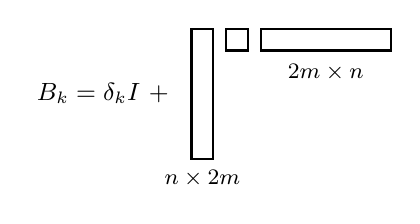
\begin{tikzpicture}[scale=0.55]
      \node[font=\small,anchor=east] at (0.1,1.5) {$B_{k}=\delta_{k}I\ +$};
      \draw[thick] (0.4,0) rectangle (0.9,3);
      \draw[thick] (1.2,2.5) rectangle (1.7,3);
      \draw[thick] (2.0,2.5) rectangle (5.0,3);
      \node[font=\footnotesize] at (0.65,-0.45) {$n\times 2m$};
      \node[font=\footnotesize] at (3.5,2.0) {$2m\times n$};
    \end{tikzpicture}\\
    {\small Figure 7.1}
  \end{minipage}\hfill
  \begin{minipage}[c]{0.58\textwidth}
    \begin{itemize}\setlength\itemsep{0.15em}
      \item The middle matrix is only $2m\times 2m$.
      \item Update: about $2mn+O(m^{3})$ operations.
        Product $B_{k}v$: $(4m+1)n+O(m^{2})$.
      \item Used in trust-region methods, L-BFGS-B, KNITRO, IPOPT.
    \end{itemize}
  \end{minipage}

  \vspace{0.4em}
  \notinbook\ IPOPT: \texttt{hessian\_approximation=limited-memory} is (7.29).
\end{frame}

\begin{frame}{SR1 in compact form; unrolling the update}
  \textbf{SR1.} With $S_{k},Y_{k},D_{k},L_{k}$ as in (7.25)--(7.27), $k$ SR1 updates (6.24) of $B_{0}$ give
  \[
    B_{k}=B_{0}+(Y_{k}-B_{0}S_{k})\big(D_{k}+L_{k}+L_{k}^{T}-S_{k}^{T}B_{0}S_{k}\big)^{-1}(Y_{k}-B_{0}S_{k})^{T} .
    \tag{7.30}
  \]
  Limited-memory SR1 is sometimes not as effective as L-BFGS: it may not produce
  positive definite approximations near a solution.

  \vspace{0.3em}
  \textbf{Unrolling.} The obvious implementation of limited-memory BFGS for $B_{k}$:
  \[ B_{k}=B_{k}^{0}+\sum_{i=k-m}^{k-1}\big[b_{i}b_{i}^{T}-a_{i}a_{i}^{T}\big] , \tag{7.33} \]
  with $a_{i},b_{i}$ from Procedure 7.6: about $\tfrac32m^{2}n$ operations, against $2mn$ for the compact form.
\end{frame}

%=====================================================================
\section{\S7.3 Sparse quasi-Newton updates}

\begin{frame}{Sparse quasi-Newton updates}
  Demand that $B_{k}$ has the same sparsity pattern as the true Hessian:
  \[ \Omega\overset{\text{def}}{=}\{(i,j)\ |\ [\hessf(x)]_{ij}\ne 0\ \text{for some $x$ in the domain of $f$}\} . \]
  \begin{align}
    \min_{B}\quad & \|B-B_{k}\|_{F}^{2}=\sum_{(i,j)\in\Omega}\big[B_{ij}-(B_{k})_{ij}\big]^{2}, \tag{7.34a}\\
    \text{subject to}\quad & Bs_{k}=y_{k},\ \ B=B^{T},\ \ \text{and}\ \ B_{ij}=0\ \text{for } (i,j)\notin\Omega . \tag{7.34b}
  \end{align}
  \begin{itemize}\setlength\itemsep{0.3em}
    \item $B_{k+1}$ is not guaranteed to be positive definite.
    \item Not scale invariant; \alert{disappointing in practice}. \readbook{pp.~185--186.}
  \end{itemize}
\end{frame}

%=====================================================================
\section{\S7.4 Partially separable functions}

\begin{frame}{Partially separable functions}
  $f$ is a sum of \textbf{element functions}, each depending on only a few components of $x$:
  \[ f(x)=\sum_{i=1}^{ne}f_{i}(x) . \tag{7.35} \]
  Example, with four element functions $f_{1},\dots,f_{4}$:
  \[
    f(x)=(x_{1}-x_{3}^{2})^{2}+(x_{2}-x_{4}^{2})^{2}+(x_{3}-x_{2}^{2})^{2}+(x_{4}-x_{1}^{2})^{2} .
    \tag{7.36}
  \]
  $f_{1}$ depends on the \emph{element variables} $x_{[1]}=(x_{1},x_{3})^{T}=U_{1}x$, where $U_{1}$ is a
  $2\times 4$ \emph{compactifying matrix}. With $\phi_{1}(z_{1},z_{2})=(z_{1}-z_{2}^{2})^{2}$, $f_{1}(x)=\phi_{1}(U_{1}x)$ and
  \[
    \gradf_{1}(x)=U_{1}^{T}\nabla\phi_{1}(U_{1}x),\qquad
    \hessf_{1}(x)=U_{1}^{T}\nabla^{2}\phi_{1}(U_{1}x)\,U_{1} .
    \tag{7.37}
  \]
\end{frame}

\begin{frame}{Quasi-Newton updating, element by element}
  \textbf{Key idea.} Do not approximate $\hessf_{1}$ ($n\times n$). Maintain a small dense
  approximation $B_{[1]}$ of $\nabla^{2}\phi_{1}$ ($2\times 2$ in the example). After a step from $x$ to $x^{+}$:
  \[
    s_{[1]}=x_{[1]}^{+}-x_{[1]},\qquad y_{[1]}=\nabla\phi_{1}(x_{[1]}^{+})-\nabla\phi_{1}(x_{[1]}),
    \tag{7.38}
  \]
  and $B_{[1]}$ is updated by BFGS or SR1. The same is done for every $\phi_{i}$. Then
  \[
    f(x)=\sum_{i=1}^{ne}\phi_{i}(U_{i}x)\ \ \eqn{7.40},
    \qquad\qquad
    B=\sum_{i=1}^{ne}U_{i}^{T}B_{[i]}U_{i}\ \ \eqn{7.41} .
  \]
  A trust-region step solves $B_{k}p_{k}=-\gradf_{k}$ \eqn{7.42} approximately by CG.
  $B_{k}$ is not assembled: the products $B_{k}v$ are computed from the $U_{i}$ and $B_{[i]}$.
\end{frame}

\begin{frame}{Partially separable updating: why it works, and its limits}
  \begin{itemize}\setlength\itemsep{0.55em}
    \item A problem of the form (7.36) with 1000 variables: each $B_{[i]}$ is $2\times 2$ and becomes
      accurate after just a few iterations. \alert{Standard BFGS or L-BFGS}, which ignore the
      structure, need many more iterations.
    \item The curvature condition $s_{[i]}^{T}y_{[i]}>0$ is not guaranteed: some $\nabla^{2}\phi_{i}$ may be
      indefinite. Remedy: SR1 updates of the element Hessians (LANCELOT).
    \item Limitations: the cost of the step computation (7.42) is comparable to the cost of
      a Newton step, and the partially separable structure can be difficult to identify.
    \item When the structure is known, it may be more efficient to compute a Newton step.
      \readbook{pp.~188--189.}
  \end{itemize}
\end{frame}

%=====================================================================
\section{Chapter 7: summary}

\begin{frame}{Chapter 7 in one table}
  \begin{center}
  \small\setlength\tabcolsep{3.5pt}
  \begin{tabular}{lllll}
    \toprule
    Method & & Uses & Main property & Software (\S7.5) \\
    \midrule
    Newton--CG, line search & Alg.~7.1 & $\hessf_{k}d$ & rate set by $\eta_{k}$ & TN/TNBC, TNPACK \\
    Newton--CG, trust region & Alg.~7.2 & $\hessf_{k}d$ & $\ge$ Cauchy decrease & LANCELOT, TRON \\
    Newton--Lanczos & (7.14) & $\hessf_{k}d$ & more robust & GLTR \\
    L-BFGS & Alg.~7.5 & $\gradf$ & linear rate & LBFGS, M1QN3 \\
    Compact $B_{k}$ & (7.29) & $\gradf$ & $B_{k}$ instead of $H_{k}$ & L-BFGS-B, IPOPT \\
    Partially separable & (7.41) & structure & rapid, robust & LANCELOT \\
    \bottomrule
  \end{tabular}
  \end{center}

  \vspace{0.2em}
  \notinbook\ In SciPy, \texttt{scipy.optimize.minimize} offers the methods \texttt{Newton-CG},
  \texttt{trust-ncg}, \texttt{trust-krylov} and \texttt{L-BFGS-B}.
\end{frame}

\begin{frame}{Three results to carry forward}
  \begin{enumerate}\setlength\itemsep{0.6em}
    \item \textbf{The forcing sequence controls the rate.} With $\|r_{k}\|\le\eta_{k}\|\gradf_{k}\|$:
      $\eta_{k}\to 0$ gives superlinear and $\eta_{k}=O(\|\gradf_{k}\|)$ quadratic convergence. Only
      Hessian--vector products are needed.
    \item \textbf{CG--Steihaug.} Started from $z_{0}=0$, the iterates grow in norm and the first
      step is the Cauchy step. The iteration stops at the trust-region boundary or at a
      direction of nonpositive curvature.
    \item \textbf{L-BFGS.} $H_{k}\gradf_{k}$ is computed from the $m$ most recent pairs $\{s_{i},y_{i}\}$ by the
      two-loop recursion, at $4mn$ multiplications. $H_{k}$ is never formed.
  \end{enumerate}

  \vspace{0.6em}
  Proved in the book: Theorem 7.3. Informal derivation: Theorems 7.1, 7.2.\\
  Stated without proof: Theorem 7.4.
\end{frame}

\begin{frame}{Homework {\normalfont\small(problem 3 is not in the book)}}
  \begin{enumerate}\setlength\itemsep{0.5em}
    \item Exercise 7.2: show that the matrix $\hat H_{k+1}$ in (7.21) is singular.
    \item Exercise 7.3: derive the formula (7.23) under the assumption that line searches
      are exact.
    \item By hand. $m=1$, $s_{k-1}=(1,0)^{T}$, $y_{k-1}=(2,1)^{T}$, $\gradf_{k}=(1,1)^{T}$, and $H_{k}^{0}=\gamma_{k}I$
      from (7.20). Run Algorithm 7.4. Check the result against $H_{k}\gradf_{k}$ with $H_{k}$ from (7.16).
    \item Exercise 7.5: write $f(x)=x_{2}x_{3}e^{x_{1}+x_{3}-x_{4}}+(x_{2}x_{3})^{2}+(x_{3}-x_{4})$ in the form (7.40).
      Give each compactifying matrix $U_{i}$.
    \item Exercise 7.1: code Algorithm 7.5 and test it on the extended Rosenbrock function
      (p.~191) from $(-1,-1,\dots,-1)^{T}$. Observe the behavior for various values of $m$.
  \end{enumerate}
\end{frame}

\end{document}
